\chapter{Exponential Integrals}\label{chap2}

AN\pageoriginale INTEGRAL OF the type
$$
\int\limits_a^bg(x)e(f(x))\,dx
$$
is called an {\bf exponential integral}. The object of various
``saddle-point theorems'' is to give the value of such an integral
approximately in terms of the possible {\bf saddle point} $x_\circ
\in(a,b)$ satisfying, by definition, the equation
$f'(x_\circ)=0$. Results of this kind can be found \eg in
\cite{key27}, Chapter IV, and in \cite{key13}, \S~2.1.

For our purposes, the existing saddle-point theorems are some-times
too crude. However, more precise results can be obtained for smoothed
exponential integrals
$$
\int\eta(x)g(x)e(f(x))\,dx,
$$
where $\eta(x)$ is a suitable smooth weight function. The present
chapter is devoted to such integrals. The main result of \S~
\ref{chap2:sec2.1} is a saddle-point theorem, and \S~
\ref{chap2:sec2.2} deals with the case when no saddle point exists.

\section[A Saddle-Point Theorem for]{A Saddle-Point Theorem for
  Smoothed Exponential Integrals}\label{chap2:sec2.1} 

It will be convenient to single out a linear part from the function
$f$, writing thus $f(x)+\alpha x$ in place of $f(x)$. Accordingly, our
exponential integral reads
\begin{equation}\label{chap2:eq2.1.1}
I=I(a,b)=\int\limits_a^b g(x)e(f(x)+\alpha x)\,dx=\int\limits_a^b
h(x)\,dx,
\end{equation}
say, where $\alpha$ is a real number.

For\pageoriginale a given positive integer $J$ and a given real number
$U>0$, we define the weight function $\eta_J(x)$ by the equation
\begin{align}
I_J &= I_J(a,b)=U^{-J}\int\limits_0^U\,du_1\cdots
\int\limits_o^U\,du_J\int\limits_{a+u}^{b-u}h(x)\,dx\label{chap2:eq2.1.2}\\
&= \int\limits_a^b\eta_J(x)h(x)\,dx,\notag
\end{align}

where $u=u_1+\cdots +u_J$. We suppose that $JU<(b-a)/2$. Also, we
define $I_\circ=I$, and interpret $\eta_\circ(x)$ as the
characteristic function of the interval $[a,b]$. Clearly $0<\eta_J
(x)\leq 1$ for $x\in(a,b)$, and $\eta_J(X)=1$ for $a+JU\leq x\leq
b-JU$. 

The following lemma gives an alternative expression for the integral
$I_J$. 
\begin{lem}\label{chap2:lem2.1}
For any $c\in(a+JU, b-JU)$ we have 
\begin{align}\label{chap2:eq2.1.3}
I_J & =(J!U^J)^{-1}\sum\limits_{j=\circ}^J\binom{J}{j}
(-1)^j\\ 
& \qquad \left\{\int\limits_{a+jU}^c(x-ajU)^Jh(x)\,
dx\int\limits_c^{b-jU}(b-jU-x)^Jh(x)\,dx\right\}.\notag
\end{align}
\end{lem}

\begin{proof}
The case $J=0$ is trivial, and otherwise the assertion can be verified
by induction using the recursion formula 
\begin{equation}\label{chap2:eq2.1.4}
I_J(a,b)=U^{-1}\int\limits_\circ^U I_{J-1}(a+u_J, b-u_J)\,du_J.
\end{equation}

For completeness we give some details of the calculations.

Supposing that \eqref{chap2:eq2.1.3} holds for the index $J-1$, we
have by \eqref{chap2:eq2.1.4}
\begin{align*}
I_J &=U^{-1}\left((J-1)!U^{J-1}\right)^{-1}\sum\limits_{j=0}^{J-1}
\binom{J-1}{j}(-1)^j\int\limits_o^U\left\{ \int\limits_{a+jU}^c
(\max(x-a -jU-\right.\\
&\left. u_J,0))^{J-1}h(x)\,dx
+\int\limits_c^{b-jU}\left(\max\left(b-jU-u_J-x,0 
\right)\right)^{J-1}h(x)\,dx\right\}\,du_J\\
&= \left(J!U^J\right)^{-1} \sum\limits_{j=0}^{J-1}\binom{J-1}{j}
(-1)^{j+1}\left\{ \int\limits_{a+(j+1)U}^c\left(x-a-(j+1)U\right)^J
h(x)\,dx\right.\\
& +\left.\int\limits_c^{b-(j+1)U}\left(b-(j+1)U-x\right)^J
h(x)\,dx \right\}+ \left(J!U^J\right)^{-1}\sum\limits_{j=0}^{J-1}\binom{J-1}{j}
(-1)^j \\
& \hspace{2.5cm} \left\{
\int\limits_{a+jU}^c(x-ajU)^Jh(x)\,dx\int\limits_c^{b-jU}(b-jU-x)^Jh(x)\,dx\right\}\\  
&= \left(J!U^J\right)^{-1}\sum\limits_{j=1}^{J-1}\left(
\binom{J-1}{j-1}+\binom{J-1}{j}\right)(-1)^j\\
& \hspace{2cm} \left\{
\int\limits_{a+jU}^c (x-ajU)^Jh(x)\,dx + \int\limits_c^{b-jU}
(b-jU-x)^Jh (x)\,dx\right\}\\
&\qquad +\left(J!U^J\right)^{-1} \left\{ (-1)^J\left(
\int\limits_{a+JU}^c (x-a-JU)^Jh(x)\,dx+\int\limits_c^{b-JU}\right.\right.\\
& \left.(b-JU-x)^J h(x)\,dx
+ \int\limits_a^c(x-a)^Jh(x)\,dx+\int\limits_c^b
(b-x)^J h(x)\,dx\right\},
\end{align*}\pageoriginale
which yields \eqref{chap2:eq2.1.3} for the index $J$.
\end{proof}

\begin{remark*}
As a corollary of \eqref{chap2:eq2.1.3}, we obtain the identity
\begin{equation}\label{chap2:eq2.1.5}
\left(J!U^J\right)^{-1}\sum\limits_{j=0}^J\binom{J}{j}(-1)^j(z-jU)^J=1.
\end{equation}
\end{remark*}

Indeed, this holds for $z=x-a$ with $a+JU\leq x\leq c$, since
$\eta_J(x)=1$ in this interval. Then, by analytic continuation,
\eqref{chap2:eq2.1.5} holds for all complex $z$. Of course,
\eqref{chap2:eq2.1.5} can also be verified directly in an elementary
way. 

Before\pageoriginale going into formulations of the saddle-point
theorems, it is convenient to list for future reference a number of
conditions on the functions $f$ and $g$.
\begin{itemize}
\item [(i)] $f(x)$ is real for $a\leq x\leq b$.
\item [(ii)] $f$ and $g$ are holomorphic in the domain
  $$
  D=\left\{z\, \big|z-x\big|<\mu(x)\quad\text{for some}\quad
  x\in[a,b]\right\}, 
  $$
  where $\mu(x)$ is a positive function, which is continuous and
  piecewise continuously differentiable in the interval $[a,b]$.
\item [(iii)] There are positive functions $F(x)$ and $G(x)$ such that
  for $|z-x|<\mu(x)$ and $a\leq x\leq b$
  \begin{align*}
    & \left|g(z)\right|\ll G(x),\\
    & \left|f'(z)\right|\ll F(x)\mu(x)^{-1}.
  \end{align*}
\item [(iv)] $f''(x)>0$ and 
  $$
  f''(x)\gg F(x)\mu(x)^{-2}
  $$
  for $a\leq x\leq b$.
\item [(v)] $\mu'(x)\ll 1$ for $a\leq x\leq b$ whenever $\mu'(x)$
  exists.
\item [(vi)] $F(x)\gg 1$ for $a\leq x\leq b$.
\end{itemize}

Since $f'(x)+\alpha$ is monotonically increasing by (iv), it has at
most one zero, say at $x_\circ$, in the interval $(a,b)$. Whenever
terms involving $x_\circ$ occur in the sequel, it should be understood
that these terms are to be omitted if $x_\circ$ does not exist.
\begin{remark*}
By Cauchy's integral formula for the derivatives of a holomorphic
function,\pageoriginale it follows from (ii) and (iii) that 
\begin{equation}\label{chap2:eq2.1.6}
\left|f^{(n)}(x)\right|\ll n!2^nF(x)\mu(x)^{-n}\quad\text{for} \quad
a\leq x\leq b, n=1, 2,\ldots
\end{equation}
Hence the conditions (iii) and (iv) together imply that
\begin{equation}\label{chap2:eq2.1.7}
f''(x)\asymp F(x)\mu(x)^{-2}\quad\text{for}\quad a\leq x\leq b. 
\end{equation}
\end{remark*}

Next we state two saddle-point theorems. The former of these, due to
F.V. Atkinson (\cite{key2}, Lemma 1), deals with the integral $I$, and
the latter is its generalization to $I_J$. Let 
\begin{equation}\label{chap2:eq2.1.8}
E_J(x)=G(x)\left(\left|f'(x)+\alpha\right|+f''(x)^{1/2}\right)^{-J-1}.
\end{equation}

In the next theorem, and also later in this chapter, the unspecified
constant $A$ will be supposed to be positive.

\begin{thm}\label{chap2:thm2.1}
Suppose that the conditions (i) - (v) are satisfied, and let $I$ be
defined as in \eqref{chap2:eq2.1.1}. Then
\begin{align}
I &= g(x_\circ)f''(x_\circ)^{-1/2}e(f(x_\circ)+\alpha x_\circ
+1/8)\label{chap2:eq2.1.9}\\ 
&\quad +o\left(\int\limits_a^bG(x)\exp(-A|\alpha|\mu(x)-AF(x))
\,dx\right)\notag\\ 
&\quad +o\left(G\left(x_\circ\right)\mu\left(x_\circ\right)F\left(
x_\circ\right)^{-3/2}\right)+o\left(E_\circ(a)\right)+o\left(E_\circ
(b)\right).\notag
\end{align}
\end{thm}

\begin{thm}\label{chap2:thm2.2}
Let $U>0, J$ a fixed nonnegative integer, $JU<(b-a)/2$, and suppose
that the conditions (i)-(vi) are satisfied. Suppose also that 
\begin{equation}\label{chap2:eq2.1.10}
U\gg \delta(x_\circ)\mu(x_\circ)F(x_\circ)^{-1/2},
\end{equation}
where $\delta(x)$ is the characteristic function of the union of the
intervals $(a,a+JU)$ and $(b-JU,b)$. Let $I_J$ be defined as in
\eqref{chap2:eq2.1.2}. Then 
\begin{align}
I_J &= \xi_J(x_\circ)g(x_\circ)f''(x_\circ)^{-1/2}e\left(f(x_\circ)
+\alpha x_\circ+1/8\right)\label{chap2:eq2.1.11}\\
&+ o\left(\int\limits_a^b(1+(\mu(x)/U)^J)G(x)\exp(-A|\alpha|\mu (x)-AF
(x)\,dx\right)\notag\\
&+o\left(\left(1+\delta(x_\circ)F(x_\circ)^{1/2}\right)G(x_\circ)\mu
(x_\circ)F(x_\circ)^{-3/2}\right)\notag\\
& +o\left(U^{-J}\sum\limits_{j=0}^J(E_J(a+jU)+E_J(b-jU))\right),\notag
\end{align}\pageoriginale
where
\begin{align}
\xi_J(x_\circ) &= 1\quad\text{for}\quad
a+JU<x_c<b-JU,\label{chap2:eq2.1.12}\\
\xi_J(x-\circ) &= \left(J!U^J\right)^{-1}\sum\limits_{j=0}^{j_1}
\binom{J}{j}(-1)^j\sum\limits_{\circ\leq\nu\leq J/2}c_\nu f''
(x_\circ)^{-\nu}(x_\circ-a-jU)^{J-2\nu}\label{chap2:eq2.1.13}
\end{align}
for $a<x_\circ\leq a+JU$ with $j_1$ the largest integer such that
$a+j_1U<x_\circ$, 
\begin{equation}\label{chap2:eq2.1.14}
\xi_J(x_\circ)=(J!U^J)^{-1}\sum\limits_{j=0}^{j_2}\binom{J}{j}(-1)^j
\sum\limits_{\circ\leq\nu\leq J/2}c_\nu
f''(x_\circ)^{-\nu}(b-jU-x_\circ)^{J-2\nu} 
\end{equation}
for $b-JU\leq x_\circ < b$ with $j_2$ the largest integer such that
$b-j_2U>x_\circ$. The $c_\nu$ are numerical constants.
\end{thm}

\begin{proof}
We follow the argument of Atkinson \cite{key2} with some modifications
caused by the smoothing. There are four cases as regards the saddle
point $x_\circ$: 1) $a+JU<x_\circ<b-JU$, 2) $x_\circ$ does not exist,
3) $a<x_\circ\leq a+JU$, 4) $b-JU\leq x_\circ <b$. Accordingly the
proof will be in four parts.
\begin{enumerate}
\item [1)] Suppose first that $a+JU<x_\circ < b-JU$. Put
$\lambda(x)=\beta\mu(x)$, where $\beta$ is a small positive
  constant. Choose $c=x_\circ$ in the expression \eqref{chap2:eq2.1.3}
  for $I_J$.

The intervals of integration in \eqref{chap2:eq2.1.3} are
replaced by the paths shown in the figure. Here $C_1, C_3, C'_3$, and
$C_5$ are, respectively,
\begin{figure}[H]
\centering{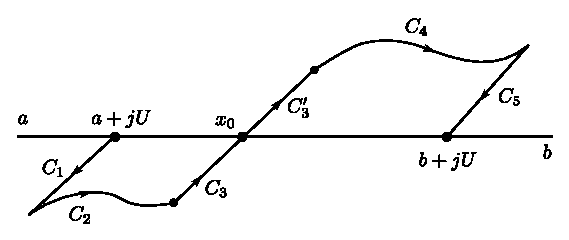
\includegraphics{fig1.eps}}
\end{figure}\pageoriginale
the line segments $[a+jU, a+jU-(1+i)\lambda(a+jU)]$,
$[x_o-(1+i)\lambda(x_o)$, $x_o]$, $[x_o,x_o
  +(1_i)\lambda(x_o)]$, and $[b-jU+(1+i)\lambda(b-jU),b-jU]$. The
curve $C_2$ is defined by $z=x-(1+i)\lambda(x), a+jU\leq x\leq
x_o$, and analogously $C_4$ is defined by $z=x+(1+i)\lambda(x),
x_o \leq x\leq b-jU$. By the holomorphicity assumption (ii) and
Cauchy's integral theorem, we have  
\begin{gather}
I_J=\left(J!U^J\right)^{-1}\sum\limits_{j=0}^J\binom{J}{j}(-1)^j
\left\{ \int\limits_{C_1+C_2+C_3}(z-a-jU)^Jh(z)
\,dz\right.\label{chap2:eq2.1.15}\\ 
+\left.\int\limits_{C'_3+C_4+C_5}(b-jU-z)^Jh(z)\,dz\right\}.\notag
\end{gather}

To estimate the modulus of $h(z)$, we need an upper bound for
$Re\{2\pi i(f(z)+\alpha z)\}$. Let $z=x+(1+i)y$, where $a\leq
x\leq b$ and $|y|\leq\lambda(x)$. By Taylor's theorem,
\begin{equation}\label{chap2:eq2.1.16}
f(z)+\alpha z=f(x)+\alpha x+(f'(x)+\alpha)(1+i)y+if''(x)y^2+
\theta(x,y), 
\end{equation}
where
$$
\theta(x,y)=\sum\limits_{n=3}^\infty\left(f^{(n)}(x)/n!\right)
((1+i)y)^n.
$$

By \eqref{chap2:eq2.1.6}, we have 
$$
|\theta(x,y)|\ll F(x)|y|^3\mu(x)^{-3},
$$\pageoriginale
so that by (iv)
$$
|\theta(x,y)|\leq\frac{1}{2}y^2f''(x)
$$
if $\beta$ is supposed to be sufficiently small. Then
\eqref{chap2:eq2.1.16} gives 
\begin{equation}\label{chap2:eq2.1.17}
Re\left\{ 2\pi i(f(z)+\alpha z)\right\}\leq -2\pi(f'(x)+\alpha)y -\pi
f''(x)y^2 
\end{equation}
for $a\leq x\leq b$ and $|y|\leq \lambda(x)$.

Consider, in particular, the case $y=sgn(f'(x)+\alpha)\lambda(x)$,
which occurs in the estimation of the integrals over $C_2$ and
$C_4$. The right hand side of \eqref{chap2:eq2.1.17} is now at most 
$$
-A|f'(x)+\alpha|\mu(x)-AF(x).
$$

In the cases $|\alpha|\geq 2|f'(x)|$ and $|\alpha|<2|f'(x)|$ this is 
$$
\leq -A|\alpha|\mu(x)-AF(x)
$$
and 
$$
\leq -AF(x)\leq -A|\alpha|\mu(x)-AF(x),
$$
respectively. Hence for $z\in C_2\cup C_4$
\begin{equation}\label{chap2:eq2.1.18}
|h(z)|\ll G(x)\exp(-A|\alpha|\mu(x)-AF(x)).
\end{equation}

The paths $C_i$ for $i=1,2,4$ and $5$ depend on $j$, so that for
clarity we denote them by $C_i(j)$. Let us first estimate the
contribution of the integrals over the $C_2(j)$ and $C_4(j)$ to
$I_J$. By the identity \eqref{chap2:eq2.1.5}, the integrands in
\eqref{chap2:eq2.1.15} combine to give simply $h(z)$ on $C_2(j) \cup
C_3\cup C'_3\cup C_4(j)$, hence in particular on $C_2(j)\cup
C_4(j)$. Thus, by \eqref{chap2:eq2.1.18} and the assumption (v),
viz. $\mu'(x)\ll 1$, the integrals in \eqref{chap2:eq2.1.15}
restricted\pageoriginale to $C_2(j)$ and $C_4(j)$ contribute
$$
\ll \int\limits_{a+JU}^{b-JU}G(x)\exp(-A|\alpha|\mu(x)-AF(x))\,dx.
$$

Integrals over the other parts of the $C_2(j)$ and $C_4(j)$ are
estimated similarly, but noting that the function in front of $h(z)$
is now $\ll 1+(\mu(x)/U)^J$. In this way it is seen that the integrals
over the $C_2(j)$ and $C_4(j)$ give together at most the first error
term in \eqref{chap2:eq2.1.11}. 

Next we turn to the integrals over the $C_1(j)$ and $C_5(j)$. By
\eqref{chap2:eq2.1.17} we have 
\begin{align*}
\int\limits_{C_1(j)}(z-a-jU)^Jh(z)\,dz & \ll G(a+jU)
\int\limits_\circ^\infty y^J\exp(-2\pi|f'(a+jU)\\
&\qquad +\alpha|y-\pi f''(a+jU)y^2)\,dy\\
& \ll E_J(a+jU),
\end{align*}
and similarly for the integrals over the $C_5(j)$. Hence these
integrals contribute the last error term in \eqref{chap2:eq2.1.11}.

Finally, as was noted above, the integrals over $C_3+C'_3$ give
together the integral
\begin{equation}\label{chap2:eq2.1.19}
K=(1+i)\int\limits_{-\lambda(x_\circ)}^{\lambda(x_\circ)}h(x_\circ+
(1+i)y)\,dy. 
\end{equation}

Applying Taylor's theorem and similar arguments as in the proof of
\eqref{chap2:eq2.1.17}, we find that for $|y|\leq\lambda(x_\circ)$
\begin{equation}\label{chap2:eq2.1.20}
g(x_o+(1+i)y)=g(x_o)+g'(x_o)(1+i)y+o\left(G(x_o)\mu
(x_o)^{-2}y^2\right),
\end{equation}
or, more crudely,
\begin{equation}\label{chap2:eq2.1.21}
g(x_\circ+(1+i)y)=g(x_\circ)+o\left(G(x_\circ)\mu(x_\circ)^{-1}
|y|\right),
\end{equation}
and analogously 
\begin{align}
& f(x_\circ+(1+i)y)+\alpha(x_\circ+(1+i)y) = f(x_\circ)+\alpha
x_\circ\label{chap2:eq2.1.22}\\
&\qquad +i f''(x_\circ)y^2+\frac{1}{6}{f''}'(x_\circ)\quad(1+i)^3y^3
+o\left(F(x_\circ)\mu(x_\circ)^{-4}y^4\right)\notag\\
&= f(x_\circ)+\alpha x_\circ+i f''(x_\circ)y^2+o\left(F(x_\circ)\mu
(x_\circ)^{-3}|y|^3\right).\label{chap2:eq2.1.23}
\end{align}\pageoriginale

Let
\begin{equation}\label{chap2:eq2.1.24}
v=\lambda(x_\circ)F(x_\circ)^{-1/3},
\end{equation}
and write $K=K_1+K_2+K_3$, where the integrals $K_1,K_2$, and $K_3$
are taken over the intervals $[-\lambda(x_\circ),-v], [-v,v]$, and
$[v,\lambda(x_\circ)]$, respectively.

First, by \eqref{chap2:eq2.1.17} we have 
\begin{align*}
K_1+K_3 & \ll G(x_\circ)\int\limits_v^\infty\exp\left(-\pi
f''(x_\circ) y^2\right)\,dy\\
& \ll G(x_\circ)v^{-1}f''(x_\circ)^{-1}\exp\left(-\pi v^2f''(x_\circ)
\right)\\
& \ll G(x_\circ)\mu(x_\circ)F(x_\circ)^{-2/3}\exp\left(-AF
(x_\circ)^{1/3}\right), 
\end{align*}
whence by (vi)
\begin{equation}\label{chap2:eq2.1.25}
K_1+K_3\ll G(x_\circ)\mu(x_\circ)F(x_\circ)^{-3/2}.
\end{equation}

The integral $K_2$, which will give the saddle-point term is evaluated
by applying \eqref{chap2:eq2.1.20} and \eqref{chap2:eq2.1.22}. The
latter implies that for $|y|\leq v$
\begin{align}
& e\left(f\left(x_\circ+(1+i)\right)+\alpha\left(x_\circ+(1+i)y
\right)\right)\label{chap2:eq2.1.26}\\
& = e\left(f(x_\circ)+\alpha x_\circ\right)\exp\left(-2\pi
f''(x_\circ)y^2\right)\times\notag\\
& \times  \Bigg\{1+\frac{1}{3}\pi i f''(x_\circ)\;(1+i)^3y^3+o\left(
F(x_\circ)\mu(x_\circ)^{-4}y^4\right)\notag\\
&\hspace{4cm} +o\left(F(x_\circ)^2\mu(x_\circ)^{-6}
y^6\right)\Bigg\};\notag
\end{align}
note that the last two terms in \eqref{chap2:eq2.1.22} are $\ll 1$ by
the choice \eqref{chap2:eq2.1.24} of\pageoriginale $v$. When this
equation is multiplied by \eqref{chap2:eq2.1.20} and the product is
integrated over the interval $[-v,v]$, the integrals of those explicit
terms involving odd powers of $y$ vanish, and we end up with 
\begin{gather}
K_2=(1+i)g(x_\circ)e\left(f(x_\circ)+\alpha x_\circ\right)
\int\limits_{-v}^v\exp \left(-2\pi f''(x_\circ)y^2\right)
\,dy\label{chap2:eq2.1.27}\\
+o\left(G(x_\circ)\int\limits_{-v}^v\exp\left(-2\pi
f''(x_\circ)y^2\right)\;\left(\mu(x_\circ)^{-2}y^2+F(x_\circ)\mu
(x_\circ)^{-4}y^4+\right.\right.\notag\\
\left.\left.F(x_\circ)^2\mu(x_\circ)^{-6}y^6\right)\,dy\right).\notag 
\end{gather}

In the main term, the integration can be extended to the whole line
with an error $\ll G(x_\circ)\mu(x_\circ)F(x_\circ)^{-3/2}$, and since 
\begin{equation}\label{chap2:eq2.1.28}
\int\limits_{-\infty}^\infty\exp\left(-cy^2\right)\,dy=(\pi/c)^{1/2}
(c>0), 
\end{equation}
the leading term in \eqref{chap2:eq2.1.27} gives the leading term in
\eqref{chap2:eq2.1.11} with $\xi(x_\circ)=1$, in accordance with
\eqref{chap2:eq2.1.12}. Further, as a generalization of
\eqref{chap2:eq2.1.28}, we have 
\begin{equation}\label{chap2:eq2.1.29}
\int\limits_{-\infty}^\infty\exp\left(-cy^2\right)y^{2\nu}\,dy= d_\nu
c^{-\nu-1/2}(c>0,\nu\geq 0)
\end{equation}
where the $d_\nu$ are certain numerical constants, and by using this
the error terms in \eqref{chap2:eq2.1.27} are seen to be $\ll
G(x_\circ)\mu(x_\circ)F(x_\circ)^{-3/2}$. 
\item [2)] Suppose next that $x_\circ$ does not exist. Then
  $f'(x)+\alpha$ is of the same sign, say positive, in the whole
  interval $(a,b)$. Let $c$ be a point in the interval $(a+JU,b-JU)$,
  write $I_J$ as in \eqref{chap2:eq2.1.3}, and transform the integrals
  over the intervals $[a+jU,c]$ and $[c,b-jU]$ using the contours
  shown in the figure, where the curvilinear part is defined by
  $z=x+(1+i)\lambda(x)$ with $a+jU\leq x\leq b-jU$. Observe that the
  integrals over the segment $[c,c+(1+i)\lambda(c)]$ cancel, by
  \eqref{chap2:eq2.1.5}. Integrals over the other parts of the
  contours are estimated as in the preceding case,\pageoriginale and
  these contribute the first and last error term in
  \eqref{chap2:eq2.1.11}. 
\begin{figure}[H]
\centering
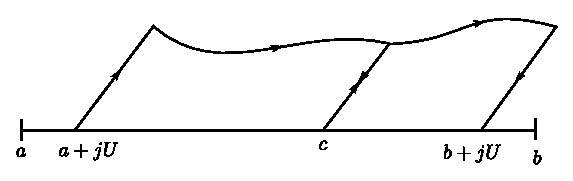
\includegraphics{fig2.eps}
\end{figure}

If $f'(x)+\alpha$ is negative, then an analogous contour is used in
the lower half-plane.
\item [3)] Consider now the case $a<x_\circ \leq a+ JU$. Again choose
$c\in (a+JU,b-JU)$. In \eqref{chap2:eq2.1.3} the integrals over
  $[c,b-jU]$ are written as in the preceding case, and likewise the
  integrals over $[a+jU,c]$ for $j>j_1$, in which case the saddle
  point $x_\circ$ does not lie in the (open) interval of
  integration. On the other hand, for $j\leq j_1$ the contour is of a
  shape similar to the first case. Only the last mentioned integrals
  require a separate treatment; the others give error terms as before.

A new complication is that the sum over $j\leq j_1$ of the integrals
over the line segment $L=[x_\circ -(1+i)\lambda(x_\circ), x_\circ
  +(1+i)\lambda(x_\circ)]$ cannot be written as an integral of $h(z)$,
but the integrals have to be evaluated separately. Other parts of the
contours do not present any new difficulties.

Thus,\pageoriginale consider the integral
\begin{equation}\label{chap2:eq2.1.30}
K=U^{-J}\int\limits_L(z-a-jU)^J h(z)\,dz.
\end{equation}

This is of the same type as the integral $K$ in \eqref{chap2:eq2.1.19}
- with $g(z)$ replaced by $U^{-J}(z-a-jU)^Jg(z)$ - so that in
principle it would be possible to apply the result of the previous
discussion as such. But then the function $G(x)$ would have to be
replaced by $U^{-J}\mu(x)^J\break G(x)$, which may become large if $J$ is
large. Therefore we modify the argument in order to prevent the error
term from becoming impracticably large.

But the first step in the treatment of the integral $K$ is as
before. Namely, let $v$ be as in \eqref{chap2:eq2.1.24}, put
$z=x_\circ +(1+i)y$, and let $K_1$ and $K_3$ be the integrals with
respect to $y$ over the intervals $[-\lambda(x_\circ),-v]$ and $[v,
\lambda(x_\circ)]$. Then $K_1+K_3$ can be estimated as before, except
that the extra factor $1+(v/U)^J$ has to be inserted. But since
$(v/U)^J \ll F(x_\circ)^{J/6}$ by \eqref{chap2:eq2.1.10} and
\eqref{chap2:eq2.1.24}, the estimate \eqref{chap2:eq2.1.25} remains
valid even for the new integrals $K_1$ and $K_3$.

The new integral $K_2$, which represents the main part of $K$, is now 
$$
K_2=(1+i)U^{-J}\int\limits_{-v}^v(x_\circ-a-jU+(1+i)y)^J h(x_\circ+
(1+i)y)\,dy.
$$

For the function $h(x_\circ+(1+i)y)$ we are going to use a somewhat
cruder approximation than before. By \eqref{chap2:eq2.1.21} and
\eqref{chap2:eq2.1.23} we have 
\begin{align}
& \quad h(x_\circ+(1+i)y)\label{chap2:eq2.1.31}\\
=& \left\{g(x_\circ)e(f(x_\circ)+\alpha x_\circ)+o\left(G(x_\circ)\mu
(x_\circ)^{-1}|y|\right)\right.\notag\\
& \left.+o\left(F(x_\circ)G(x_\circ)\mu(x_\circ)^{-3}
|y|^3\right)\right\}\times \exp\left(-2\pi f''(x_\circ)y^2\right).\notag
\end{align}

Since\pageoriginale by \eqref{chap2:eq2.1.29}, \eqref{chap2:eq2.1.10},
and (iv)
\begin{align*}
& U^{-J}\int\limits_{-v}^v\left(U^J+|y|^J\right)|y|^\nu\exp\left(-2\pi
f''(x_\circ)y^2\right)\,dy\\
& \ll f''(x_\circ)^{-(\nu+1)/2}+U^{-J}f''(x_\circ)^{-(\nu+J+1)/2}\\
& \ll \mu(x_\circ)^{\nu+1}F(x_\circ)^{-(\nu+1)/2}
\end{align*}
the contribution of the error terms in \eqref{chap2:eq2.1.31} to $K_2$
is $\ll G(x_\circ)\break\mu(x_\circ)$ $F(x_\circ)^{-1}$. Hence
{\fontsize{10}{12}\selectfont
\begin{align*}
K_2 &= \sqrt{2}g(x_\circ)e(f(x_\circ)+\alpha x_\circ+1/8)U^{-J}
\int\limits_{-v}^v \left(x_\circ-a-jU+(1+i)y\right)^J\\
& \quad\exp\left(-2\pi f''(x_\circ)y^2\right)\,dy
+o\left(G(x_\circ)\mu(x_\circ)F(x_\circ)^{-1}\right)\\ 
&= \sqrt{2}g(x_\circ)e\left(f(x_\circ)+\alpha x_\circ+1/8\right)U^{-J}
\sum\limits_{0\leq\nu\leq J/2}(x_\circ-a-jU)^{J-2\nu}\times\\
&\qquad \times (1+i)^{2\nu}\binom{J}{2\nu}\int\limits_{-v}^vy^{2\nu}\exp
\left(-2\pi f''(x_\circ)y^2\right)\,dy\\
& \qquad +o\left(G(x_\circ)\mu(x_\circ) F(x_\circ)^{-1}\right). 
\end{align*}}

As before, the integrals here can be extended to the whole real line
with a negligible error. Then, evaluating the new integrals by
\eqref{chap2:eq2.1.29} we find that with 
$$
c_\nu=2^{-\nu}\pi^{-\nu-1/2}(1+i)^{2\nu}\binom{J}{2\nu}d_\nu
$$
and with $\xi(x_\circ)$ as in \eqref{chap2:eq2.1.13}, the resulting
expression for $I_J$ is as in \eqref{chap2:eq2.1.11}.
\item [4)] The remaining case $b-jU\leq x_\circ <b$ is analogous to
  the preceding one.
\end{enumerate}
\end{proof}

\begin{remark*}
If $f$ satisfies the conditions of Theorem \ref{chap2:thm2.1} and
\ref{chap2:thm2.2} except that $f''(x)$ is negative in the interval
$[a,b]$, then the results hold with\pageoriginale the minor
modifications that in the main term the factor $e(f(x_\circ)+\alpha
x_\circ +1/8)$ is to be replaced by $e(f(x_\circ)+\alpha x_\circ
-1/8)$, and $|f''(x_\circ)|$ should stand in place of $f''(x_\circ)$. 
\end{remark*}

\section{Smoothed Exponential Integrals without a Saddle
  Point}\label{chap2:sec2.2} 

Theorem \ref{chap2:thm2.2} covers also the case of exponential
integrals $I_J$ without a saddle point. However, in applications, the
condition (iv) on $f''$ may not be fulfilled. Nevertheless, if the
assumption of $f'$ is strengthened, then no assumption on $f''$ is
needed. The next theorem is a result of this kind.

\begin{thm}\label{chap2:thm2.3}
Suppose that the functions $f$ and $g$ satisfy the conditions (i) and
(ii) in the preceding section, with $\mu(x)=\mu$, a constant. Suppose
also that
\begin{align}
& |g(z)|\ll G\quad\text{for}\quad z\in D,\label{chap2:eq2.2.1}\\
& |f'(x)|\asymp M\quad\text{for}\quad a\leq x\leq
b,\label{chap2:eq2.2.2}\\
\intertext{and}
& |f'(z)|\ll M\quad\text{for}\quad z\in D.\label{chap2:eq2.2.3}
\end{align}

Let $I_J$ be as in \eqref{chap2:eq2.1.2} with $\alpha =0$ and $0 < JU
< (b-a)/2$. Then 
\begin{equation}\label{chap2:eq2.2.4}
I_J\ll U^{-J}GM^{-J-1}+\left(\mu^JU^{1-J}+b-a\right)Ge^{-AM_\mu}.
\end{equation}
\end{thm}

\begin{proof}
By \eqref{chap2:eq2.2.2}, the function $f'(x)$ cannot change its sign
in the interval $[a,b]$. Suppose, to be specific, that $f'(x)$ is
positive. By \eqref{chap2:eq2.2.3} and Cauchy's integral formula we
have 
$$
|f^{(k)}(x)|\ll k!M(\mu/2)^{-k+1}\quad\text{for}\quad k=1,2,\ldots
\quad\text{and}\quad a\leq x\leq b.
$$

Then, by \eqref{chap2:eq2.2.2} and Taylor's theorem, it is seen that 
\begin{equation}\label{chap2:eq2.2.5}
Re(2\pi i f(z))< -AMy
\end{equation}\pageoriginale
for $z=x+yi,a\leq x\leq b$, and $0\leq y\leq\beta\mu=\lambda$, where
$\beta$ is a sufficiently small positive constant.
\end{proof}

Now, for a proof of \eqref{chap2:eq2.2.4}, the integral $I_J$ is
written as in \eqref{chap2:eq2.1.3}, where the intervals $[a+jU,c]$
and $[c,b-jU]$ are deformed to rectangular contours respectively with
vertices $a+jU, a+jU+i\lambda, c+i\lambda$, and $c$, or $c,
c+i\lambda, b-jU+i\lambda$, and $b-jU$. Then \eqref{chap2:eq2.2.4}
follows easily by \eqref{chap2:eq2.2.1}, \eqref{chap2:eq2.2.5} and
\eqref{chap2:eq2.1.5}. 

\bigskip


\section*{Notes}

In the saddle-point lemma of Atkinson (Lemma 1 in \cite{key2}), the
assumptions on the functions $F$ and $\mu$ are weaker than those in
Theorem \ref{chap2:thm2.2}, for the conditions (v) and (vi) are
missing. Actually we posed these just for simplicity. On the other
hand, one of the conditions in  \cite{key2} is stronger than ours, for
in place of (iv) there is an upper bound for $f'' (z)^{-1}$ for $z \in
D$. However, in the proof this is needed only on the real interval $[a,b]$,
in which case it coincides with (iv).

The complications that arose in Theorem \ref{chap2:thm2.2} when
$x_\circ$ lies near $a$ or $b$ seem inevitable, for then the integrand
is almost stationary near $a$ or $b$, and consequently there is not so
much to be gained by smoothing.

The case $J=1$ of Theorem \ref{chap2:thm2.3} is Lemma 2 in
\cite{key16} and Lemma 2.3 in \cite{key13}. Our proof is not a direct
generalization of that in \cite{key16} which turned out to become
somewhat tedious for general $J$.

Theorems\pageoriginale \ref{chap2:thm2.2} and \ref{chap2:thm2.3} may
be useful in problems in which the standard results (corresponding to
$J=0$) on exponential integrals are not accurate enough. An example of
such an application is the improvement of the error terms in the
approximate functional equations for $\zeta^2(s)$ and $\varphi(s)$ in
\cite{key19}. 

The parameters $U$ and $J$, which determine the smoothing, can be
chosen differently at $a$ and $b$. Such a version of Theorem
\ref{chap2:thm2.2} is given in \cite{key19}, and the proof is
practically the same. The corresponding smoothed integrals is of the
type
$$
U^{-J}V^{-K}\int\limits_\circ^U\,du_1\cdots\int\limits_\circ^U\,du_J
\int\limits_\circ^V \,dv_1\cdots\int\limits_\circ^V\,dv_K
\int\limits_{a+u}^{b-v} h(x)\,dx,
$$
where $u=u_1+\cdots+u_J$ and $v=v_1+\cdots+ v_K$. For $U=V$ and $J=K$,
this amounts to the integral $I_J$ in \eqref{chap2:eq2.1.2}. 

